\section{Community Detection}
\label{sec:CD}

The topology shifts in Section~\ref{sec:NC}---shorter paths, reshuffled centrality rankings---raise a structural question one level up: do BC's added edges reorganise community membership, and does that reorganisation track disciplinary boundaries?  We run three algorithms on $G_{Cit}$ and $G_{BC}$, validating the resulting partitions against FOS labels at L2 macro-domain and L4 sub-discipline granularity.

\subsection{Ensemble Stabilisation}
\label{subsec:cd:stabilisation}

All three algorithms are stochastic; we stabilise each via an \emph{ensemble-plus-medoid} protocol---run the algorithm $N$ times, compute pairwise NMI across all runs, and select the partition with the highest mean NMI to all others (the medoid).

\begin{itemize}

  \item \textbf{Leiden}~\cite{traag2019louvain} uses \texttt{RBConfiguration}\allowbreak\texttt{VertexPartition}, avoiding the resolution limit of standard modularity~\cite{fortunato2007resolution}.  We sweep $\gamma$ over 30 log-spaced values in $[0.05,\,10]$ with a 100-run ensemble at each point, recording non-trivial community count ($\geq 20$ nodes) in the medoid.  Both graphs show a stable plateau: $\gamma \in [0.05,\,0.578]$ for $G_{Cit}$, $[0.05,\,0.472]$ for $G_{BC}$.  We fix $\gamma_{\text{common}} = 0.154$ from the plateau intersection, trading per-graph optimality for comparability.

  \item \textbf{InfoMap}~\cite{rosvall2008maps} minimises map-equation codelength for a random walker and requires no resolution parameter. $G_{Cit}$ enters as directed and unweighted; $G_{BC}$ as undirected and weighted.  We run a 100-run ensemble and select the medoid.

  \item \textbf{ANGEL}~\cite{rossetti2019exorcising} is the only overlap-aware method.  We calibrate \texttt{threshold} and \texttt{min\_community\_size} by sweeping an $11\times 4$ grid (threshold $\in [0.3,\,0.8]$, min\_size $\in [4,\,7]$) on both graphs and selecting the configuration that best scores coverage, overlap rate, and community count via a composite utility function.  The selected configuration is threshold\,$=0.45$, min\_size\,$=4$.  The ensemble uses 30 runs (reduced from 100: ${\sim}640$\,s per BC run); the medoid is selected via NMI on crisp projections, assigning multi-member nodes to the community containing the most of their neighbours.
\end{itemize}

Table~\ref{tab:cd-summary} confirms that all three methods are stable ($\mu_{\text{NMI}} \geq 0.91$).  InfoMap on $G_{BC}$ shows the widest spread ($\sigma = 0.037$)---the denser graph introduces more flow-routing ambiguity for the random walker.

\subsection{Community Structure and Quality}
\label{subsec:cd:results}

FOS L4 labels cover 44\,317 of 57\,603 nodes ($76.9\%$); the remaining $23.1\%$ introduces uncertainty in any disciplinary classification that follows.  The corpus is biomedical-dominant: medical and health sciences account for $49\%$ of labelled nodes, followed by natural sciences ($36\%$) and engineering ($21\%$; percentages exceed $100\%$ because nodes carry multiple labels).

\begin{table}[t]

  \centering\footnotesize
  \resizebox{\linewidth}{!}{%
  \begin{tabular}{@{}ll cccc cccc@{}}
    \toprule
     & & \multicolumn{4}{c}{Ensemble stability}
       & \multicolumn{4}{c}{Medoid partition} \\
    \cmidrule(lr){3-6}\cmidrule(l){7-10}
    Algorithm & Graph
      & Runs & $\mu_{\text{NMI}}$ & $\sigma$ & Medoid
      & \#Comm. & Med. & Mean & Largest \\
    \midrule
    Leiden  & $G_{Cit}$ & 100 & 0.941 & 0.007 & 0.952 & 1\,533 &  2 & 35.9 &  4\,520 \\
    Leiden  & $G_{BC}$  & 100 & 0.934 & 0.011 & 0.946 & 1\,210 &  2 & 47.6 &  9\,145 \\
    \midrule
    InfoMap & $G_{Cit}$ & 100 & 0.941 & 0.009 & 0.954 & 1\,496 &  3 & 45.7 & 19\,750 \\
    InfoMap & $G_{BC}$  & 100 & 0.910 & 0.037 & 0.934 & 1\,174 &  3 & 55.4 & 22\,940 \\
    \midrule
    ANGEL   & $G_{Cit}$ &  30 & 0.967 & 0.002 & 0.969 & 1\,527 &  9 & 25.4 &  1\,724 \\
    ANGEL   & $G_{BC}$  &  30 & 0.964 & 0.002 & 0.966 & 1\,514 & 10 & 31.3 &  3\,321 \\
    \bottomrule
  \end{tabular}%
  }
    \caption{Ensemble stability and medoid partition statistics.
           $\mu_{\text{NMI}}$: mean pairwise NMI across runs;
           Medoid: that run's mean NMI to all others.
           Leiden: $\gamma = 0.154$; ANGEL: threshold $= 0.45$,
           min\_size $= 4$.  Med.: median community size.}
  \label{tab:cd-summary}
\end{table}

\begin{figure}[t]
  \centering
  \begin{subfigure}[b]{0.15\textwidth}
    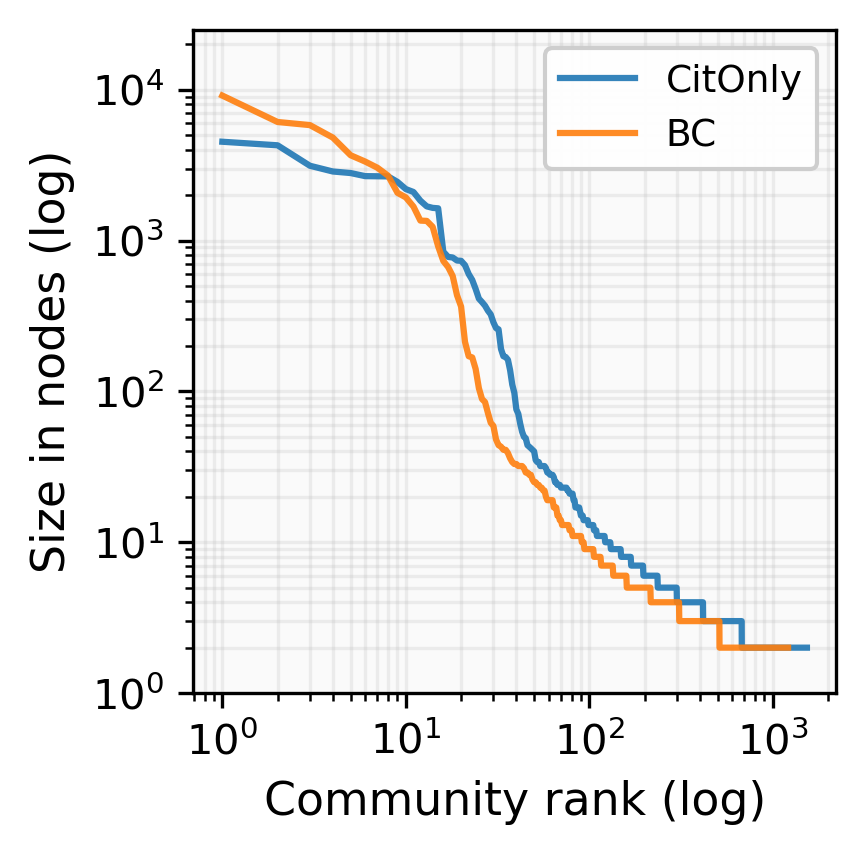
\includegraphics[width=\textwidth]{img/C_leiden_size_distribution.png}
    \caption{Leiden}
    \label{fig:dist-leiden}
  \end{subfigure}
  \hfill
  \begin{subfigure}[b]{0.15\textwidth}
    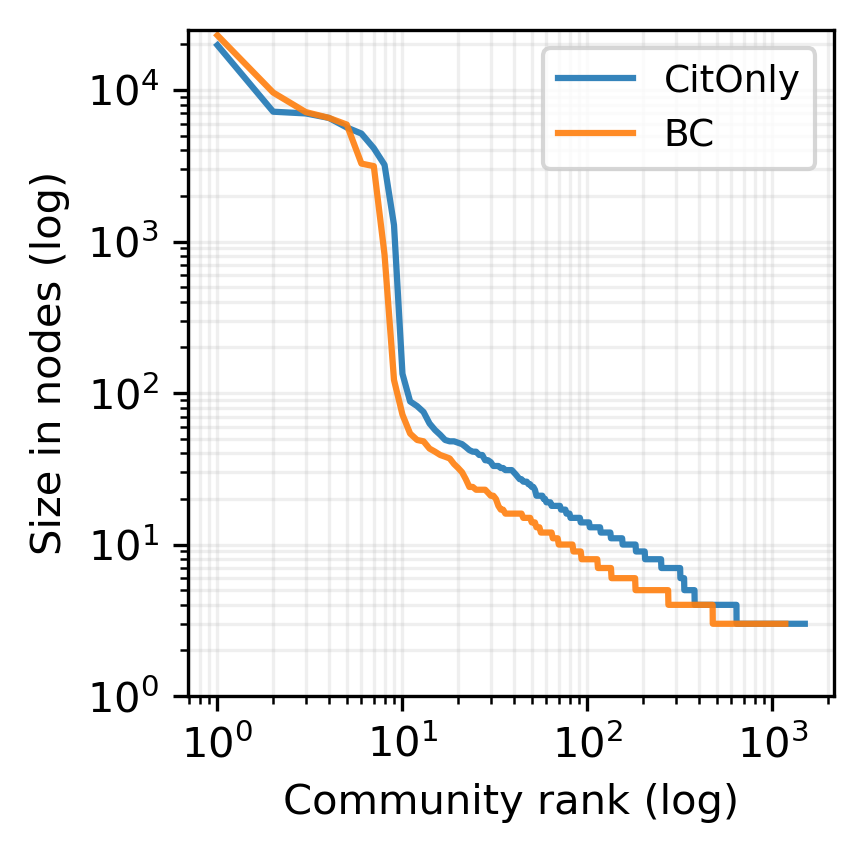
\includegraphics[width=\textwidth]{img/C_infomap_size_distribution.png}
    \caption{InfoMap}
    \label{fig:dist-infomap}
  \end{subfigure}
  \hfill
  \begin{subfigure}[b]{0.15\textwidth}
    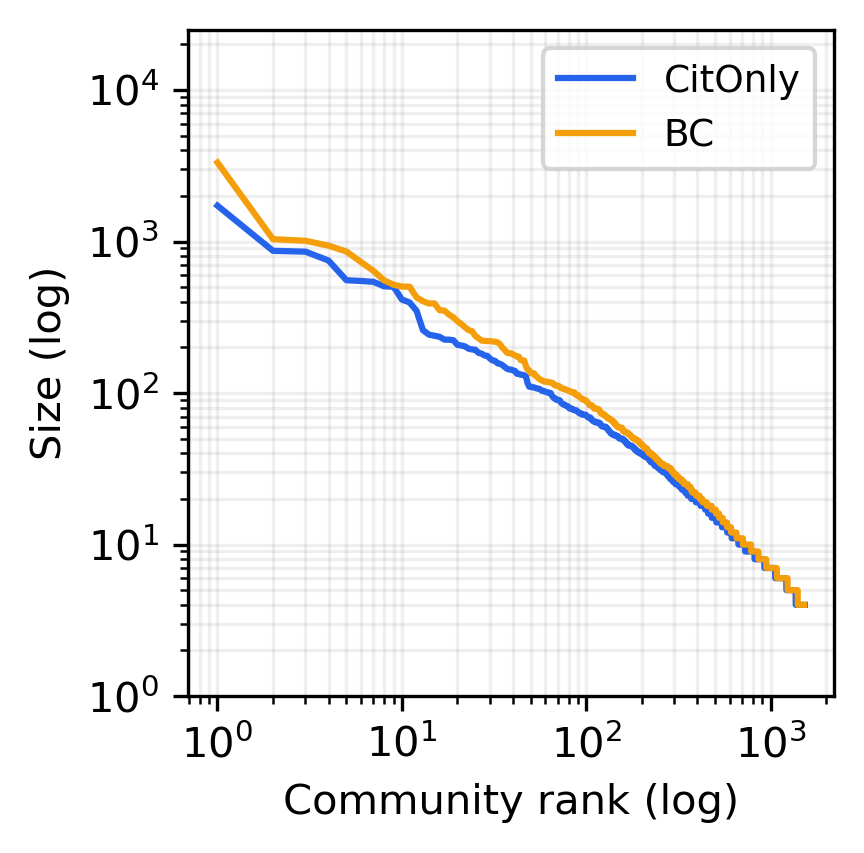
\includegraphics[width=\textwidth]{img/C_angel_size_distribution.png}
    \caption{ANGEL}
    \label{fig:dist-angel}
  \end{subfigure}
  \caption{Community size distributions (medoid partitions).}
  \label{fig:size-dist}
\end{figure}

Leiden and InfoMap agree: BC reduces community count by ${\sim}21\%$ (Table~\ref{tab:cd-summary}).  ANGEL barely moves ($-0.9\%$) because it resolves ambiguity through overlap rather than merging---its largest community nearly doubles ($1\,724 \to 3\,321$), but the total count stays flat.  Median size stays at 2--3 for the crisp methods on both graphs, reflecting the heavy tail typical of citation networks: most communities are tiny and unaffected by BC.  The consolidation happens in the upper tail---Leiden needs 9 communities to cover 50\% of nodes on $G_{Cit}$ but only 5 on $G_{BC}$.

We track what each large $G_{Cit}$ community ($\geq 20$ nodes) becomes on $G_{BC}$.  Leiden registers 18 merge events.  InfoMap concentrates its merges into only 5 events, the largest of which absorbs 10 components into a single community of 19\,664 nodes.  ANGEL stays largely stable (76\%), absorbing change through overlap. Both crisp methods retain measurable modularity on $G_{BC}$ ($Q = 0.681$ for Leiden, $0.597$ for InfoMap)---a substantial drop from $G_{Cit}$ ($Q = 0.939$, $0.837$) that reflects the density tripling, not structural collapse.

At 19\,664 nodes, one InfoMap community covers roughly 36\% of the network; assigning a third of all papers to a single group limits discriminative value regardless of internal coherence.  BC pushes it further to 22\,940 nodes, reinforcing the coarseness already present on $G_{Cit}$.

Semantic purity is measured as normalised Shannon entropy $\hat{H} = H / \log_2 k$ over FOS labels per community ($\geq 10$ nodes); $\hat{H} \to 0$ is pure, $\hat{H} \to 1$ is uniform.  Leiden's L4 entropy rises slightly on $G_{BC}$ ($\bar{H}: 0.612 \to 0.631$)---consistent with cross-disciplinary merges broadening composition. InfoMap moves in the opposite direction ($\bar{H}: 0.683 \to 0.627$), alongside a sharp drop in qualifying communities (182 $\to$ 81)---the partition consolidates rather than diversifies.  Both graphs yield comparable FOS coherence under any given algorithm; BC reshapes community granularity more than disciplinary composition.

\subsection{Cross-Algorithm Synthesis}
\label{subsec:cd:synthesis}

For each of the 18 Leiden merge events (components $\geq 20$ nodes), we check whether InfoMap and ANGEL independently group the same nodes, defining confirmation as $\geq 50\%$ overlap with one community. InfoMap confirms almost every merge (median overlap $\geq 0.98$, both INTRA and CROSS).  ANGEL does not---only 1 of 18 reaches $3/3$ consensus; its median overlap stays at $0.14$ for CROSS and $0.30$ for INTRA, reflecting fragmentation rather than disagreement.  Fifteen of 18 merges ($83\%$) are cross-disciplinary at FOS L4.

To test whether merge zones are more disciplinarily concentrated than their surroundings, we compute Gini impurity $G_I = 1 - \sum_k p_k^2$ and compare it to a multi-hop neighbourhood null (1\,000 permutations).

No merge is testable at hop 1.  Significance emerges at hop 2 (4/7 testable merges, all CROSS) and strengthens at hop 3 (13/16, including the first INTRA).  BC creates structures that become distinguishable from their surroundings only at mesoscopic scale; locally, they blend into the same disciplinary landscape.

A complementary FOS gap analysis counts how often sub-discipline pairs co-occur within the same community in $G_{Cit}$ vs $G_{BC}$.  206 pairs show a positive gap; 55 are entirely new.  But a permutation test (1\,000 shuffles preserving community sizes) finds none significant---all p-values equal $1.000$.
This is the key negative result: the co-occurrence signal is indistinguishable from a random size-preserving partition.


\paragraph{Caveats.}
The $83\%$ CROSS ratio is conditioned on $\gamma = 0.154$, which sits at the lower end of the plateau and produces relatively large communities that span multiple FOS L4 labels \emph{before} any merge, biasing classification toward CROSS.  At higher $\gamma$, the same consolidation would register as more INTRA.  The direction of BC's effect---fewer communities, larger merge zones---is robust across the plateau; the INTRA/CROSS proportion is resolution-dependent, not an absolute structural property.  $23.1\%$ of nodes lack FOS labels; the shared $\gamma_{\text{common}}$ sacrifices per-graph optimality; and ANGEL's 30-run ensemble provides less stabilisation than the other methods, though its tight NMI spread ($\sigma = 0.002$) suggests this is not limiting.